\chapter{Implementation}
\label{chapter:Implementation}	
The previous chapter introduced the fundamental concepts and ideas the are used in this project. This chapter describes how these are actually put to use, with details of all four sections of the workflow pipeline: starting from a CAD geometry input, obtaining a voxelized input for the topology optimizer, extracting the surface from the optimized voxel grid, to fitting smooth, optimally sized curves through it.
\todourgent[inline,author=Benni]{where to put licencing and link to git repo?}

\section{CADO: Computer Aided Design Optimization Tool}
CADO is the tool of choice to realize a one click CAD-to-Topology-Optimization-back-to-CAD experience. With CADO, the user only has to select the input file on which to apply the topology optimization and set the parameters which for example define the resolution or refinement level. By executing the \texttt{Run} command the tool starts the pipeline illustrated in \autoref{fig:pipeline}: 

From the given geometry (a) we start off by voxelizing (b). Next, topology optimization is applied (c) and the control points are computed (d). After computing the surface (e), finally, the boolean operation is executed and the final geometry is received (f). All of this happens in the background. To get a better insight into the implementation, in the next sections we explain the different steps in more detail.
\begin{figure}[ht]
\begin{center}
		\begin{tikzpicture}[remember picture,auto,
    block/.style={
      rectangle,
      draw=blue,
      thick,
      fill=blue!20,
      text width=5em,
      align=center,
      rounded corners,
      minimum height=2em
    },
    block1/.style={
      rectangle,
      draw=blue,
      thick,
      fill=blue!20,
      text width=5em,
      align=center,
      rounded corners,
      minimum height=2em
    },
    line/.style={
      draw,thick,
      -latex',
      shorten >=2pt
    },
    cloud/.style={
      draw=red,
      thick,
      ellipse,
      fill=red!20,
      minimum height=1em
    }]
        \node [anchor=north,inner sep=0pt] [xshift=-4cm,yshift=0.7cm,inner sep=0pt](N1)
                {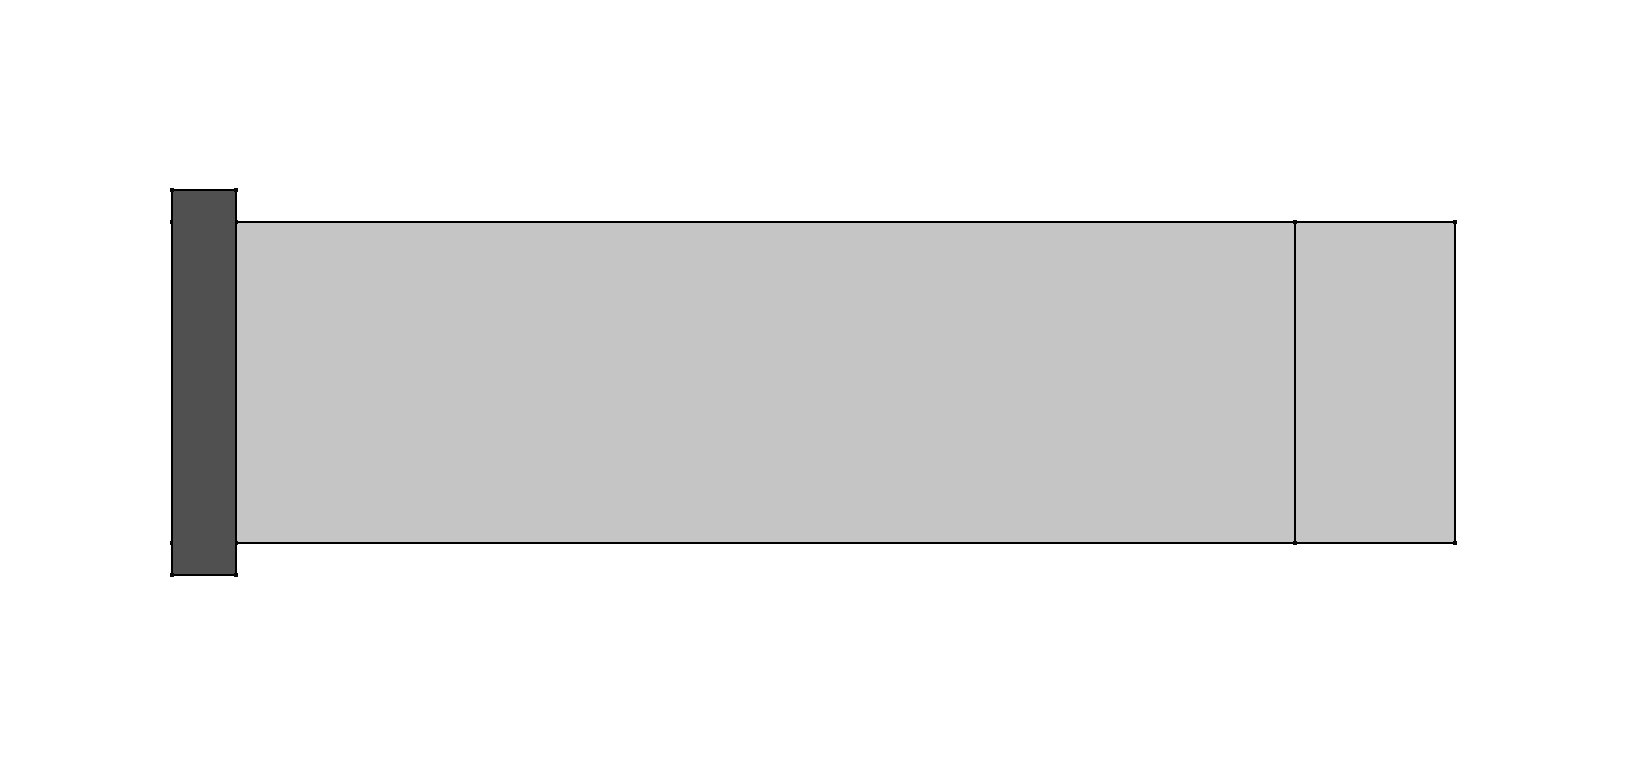
\includegraphics[scale=0.1]{Pictures/CADO_Overview/Back2CAD1.png}};
        \node [below =of N1,inner sep=0pt] [xshift=0cm,yshift=-0cm,inner sep=0pt](N5)
				{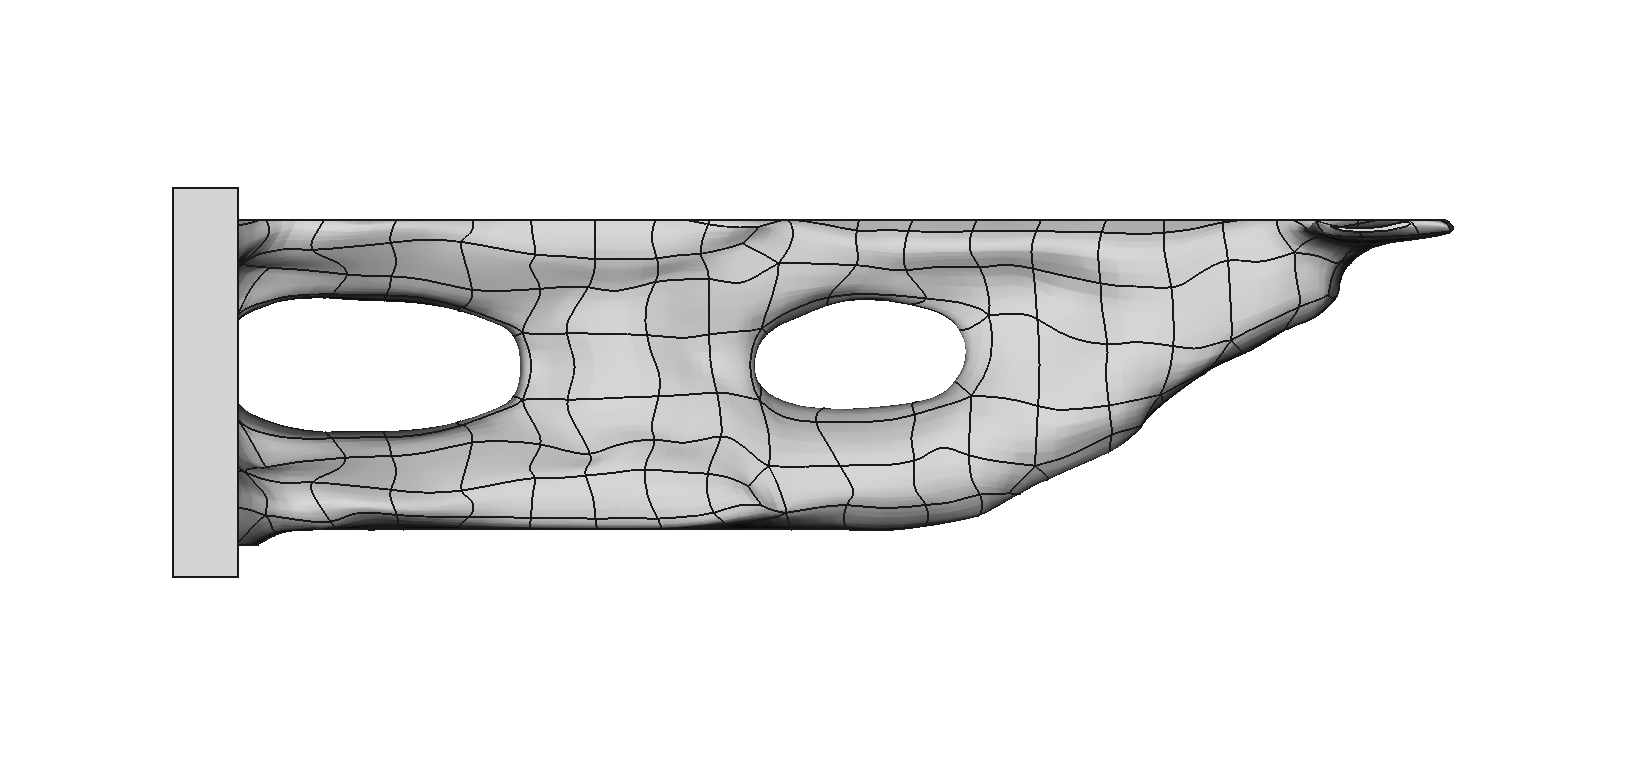
\includegraphics[scale=0.1]{Pictures/CADO_Overview/Back2CAD6.png}};
      	%\path[thick, ->,] (N5) edge [bend left] (N1); %node[yshift=-1.8cm, xshift = -0.1cm]{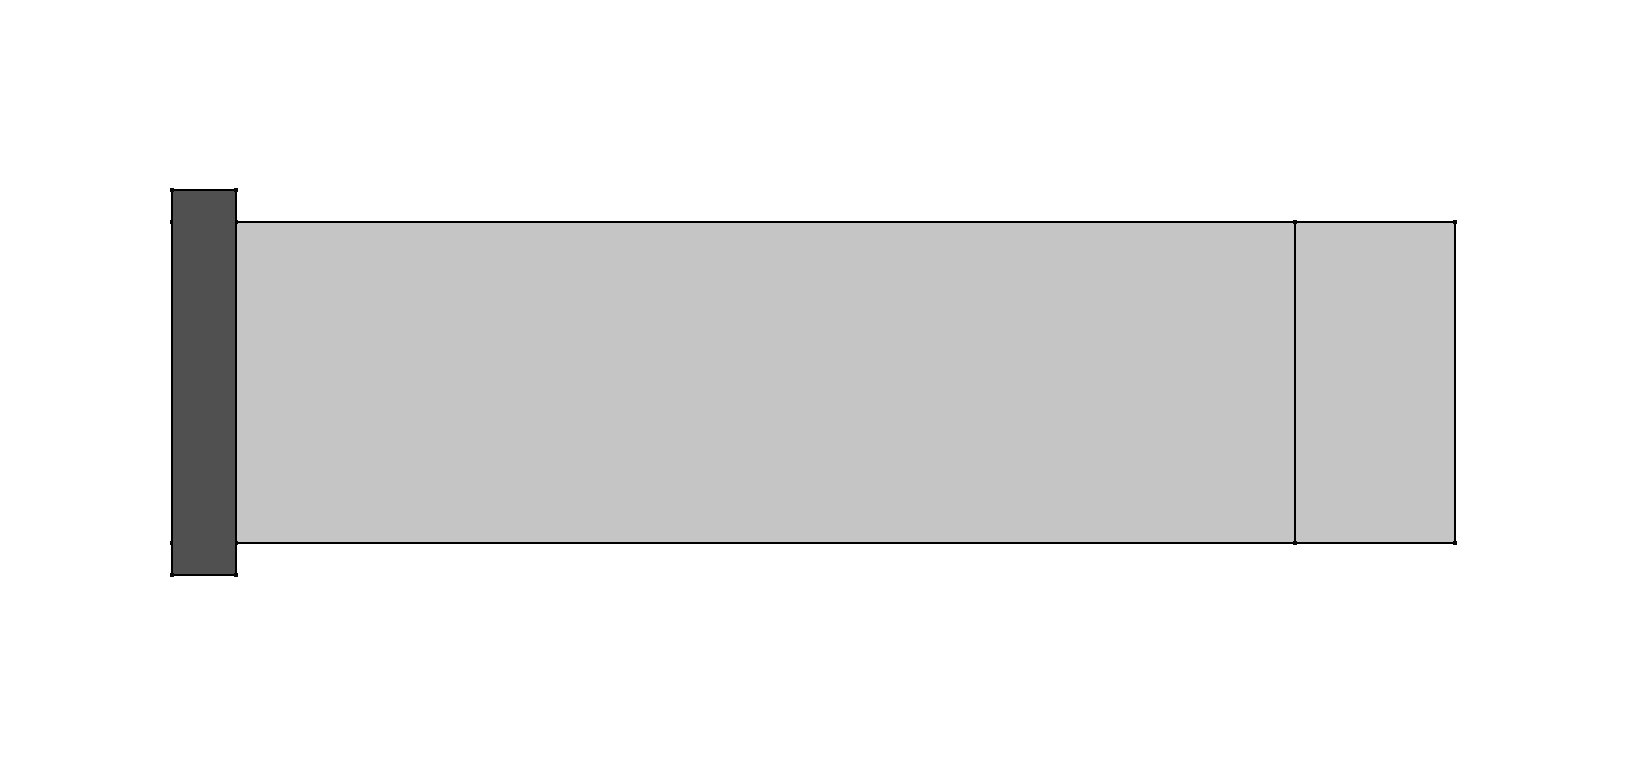
\includegraphics[scale=0.1]{Pictures/CADO_Overview/Back2CAD1.png}};
        \node [right =of N1,inner sep=0pt] [xshift=-1cm,yshift=3cm, inner sep=0pt](N2)             
                {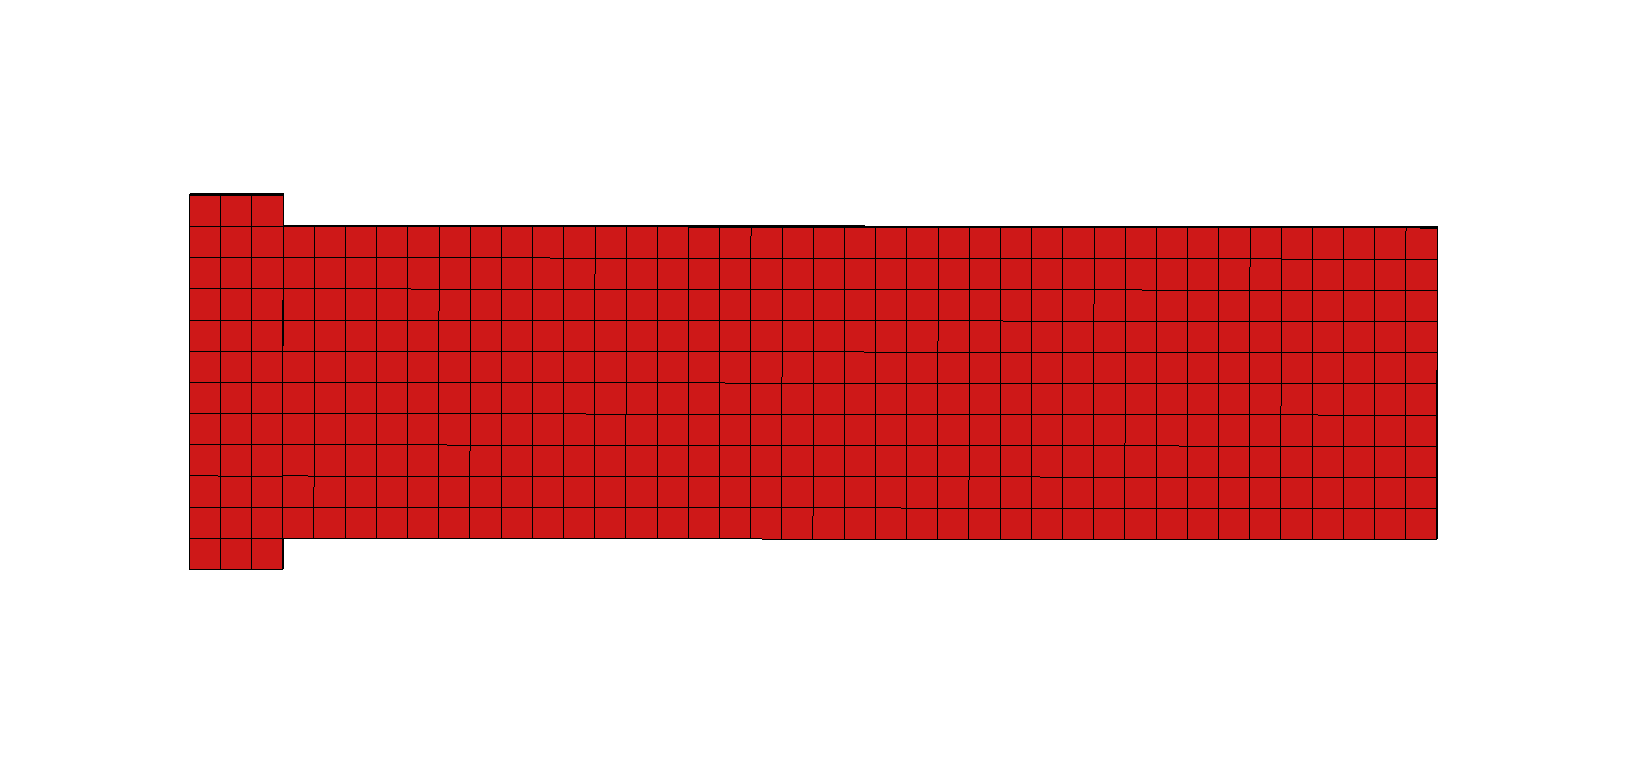
\includegraphics[scale=0.1]{Pictures/CADO_Overview/Back2CAD2.png}};
        \path[thick, ->] (N1) edge [bend left] (N2) node[yshift=0cm, xshift = -2.7cm]{(a)};
        \node [right =of N2,inner sep=0pt] [xshift=-1cm,yshift=-3cm, inner sep=0pt](N3) 
                {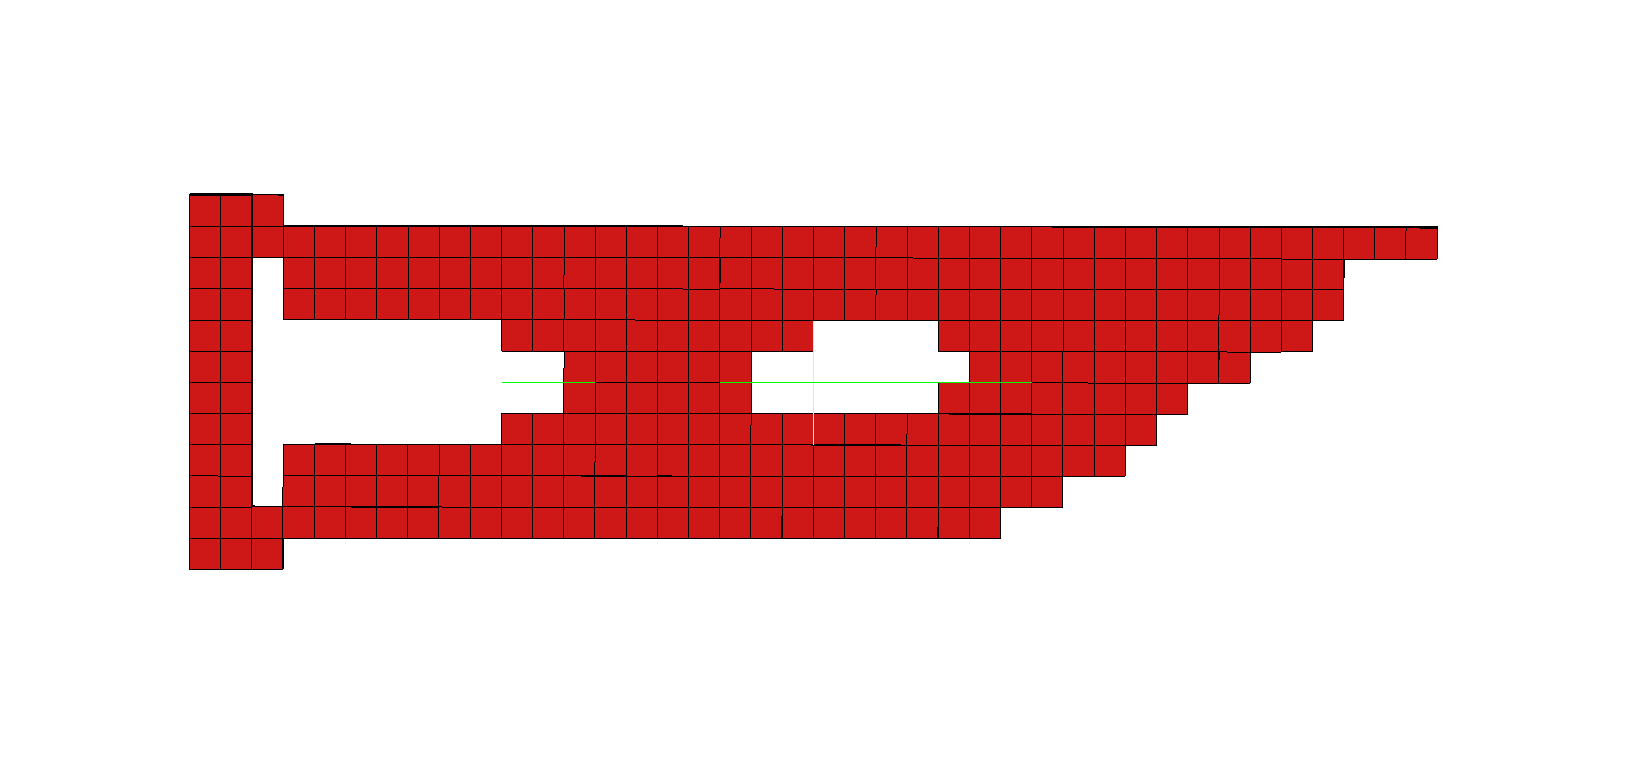
\includegraphics[scale=0.1]{Pictures/CADO_Overview/Back2CAD3.png}};
        \path[thick, ->] (N2) edge [bend left] (N3) node[yshift=1cm, xshift = 0.1cm]{(b)};
        \node [below =of N3,inner sep=0pt] [xshift=0cm,yshift=-0cm, inner sep=0pt](N4)
                {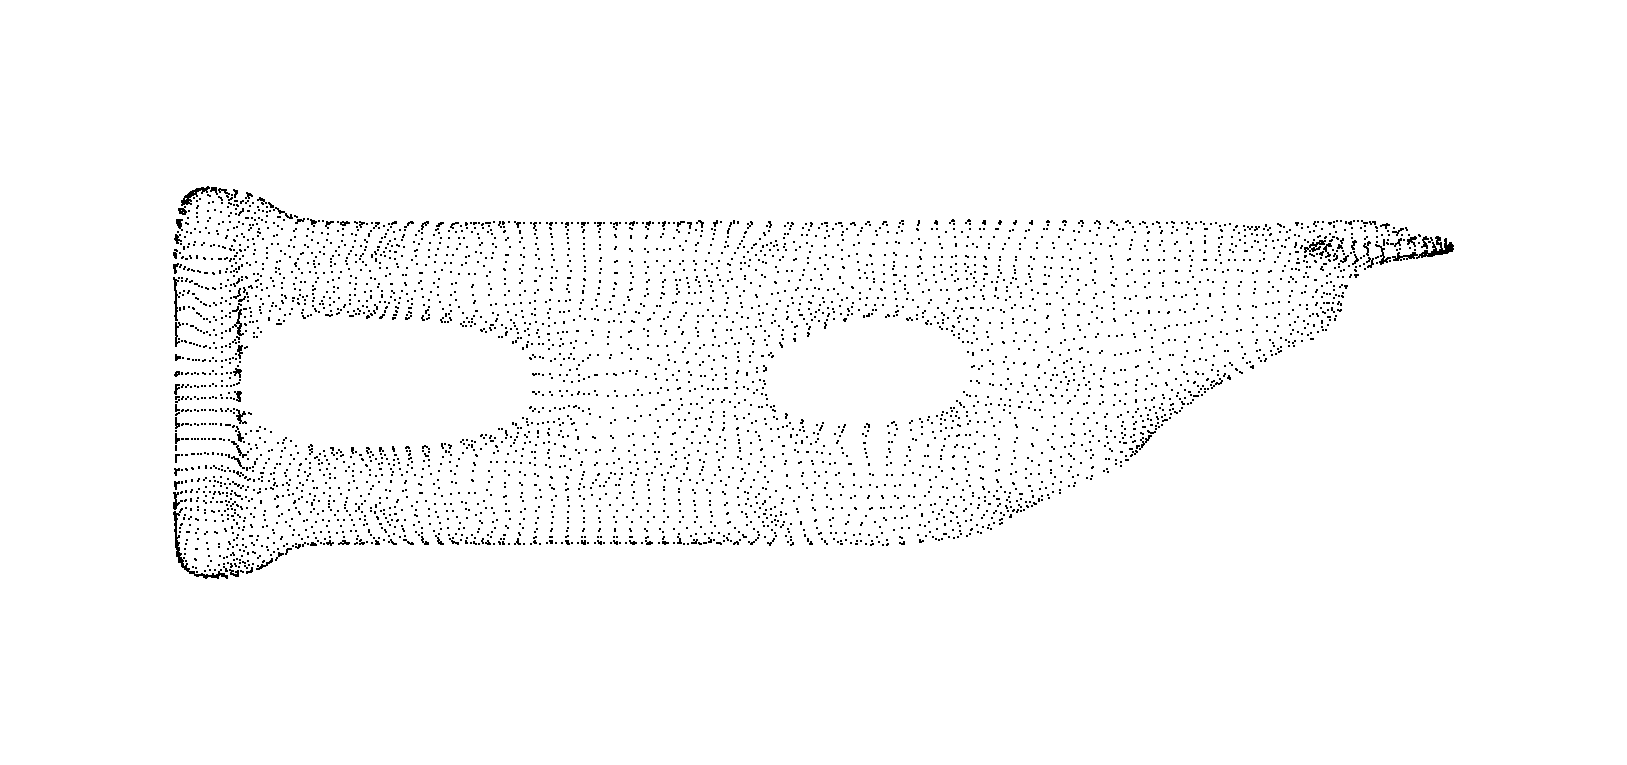
\includegraphics[scale=0.1]{Pictures/CADO_Overview/Back2CAD4.png}};
        \coordinate (N31) at (-0.7,-1);
        \coordinate (N32) at ($(N3)+(N31)$);
        \coordinate (N41) at (-0.7,1);
        \coordinate (N42) at ($(N4)+(N41)$);
        \draw[thick, ->] (N32) -- (N42) node[yshift=2.8cm, xshift = 3.4cm]{(c)};
        \node [right =of N5,inner sep=0pt] [xshift=-0.7cm,yshift=-3cm, inner sep=0pt](N6)
                {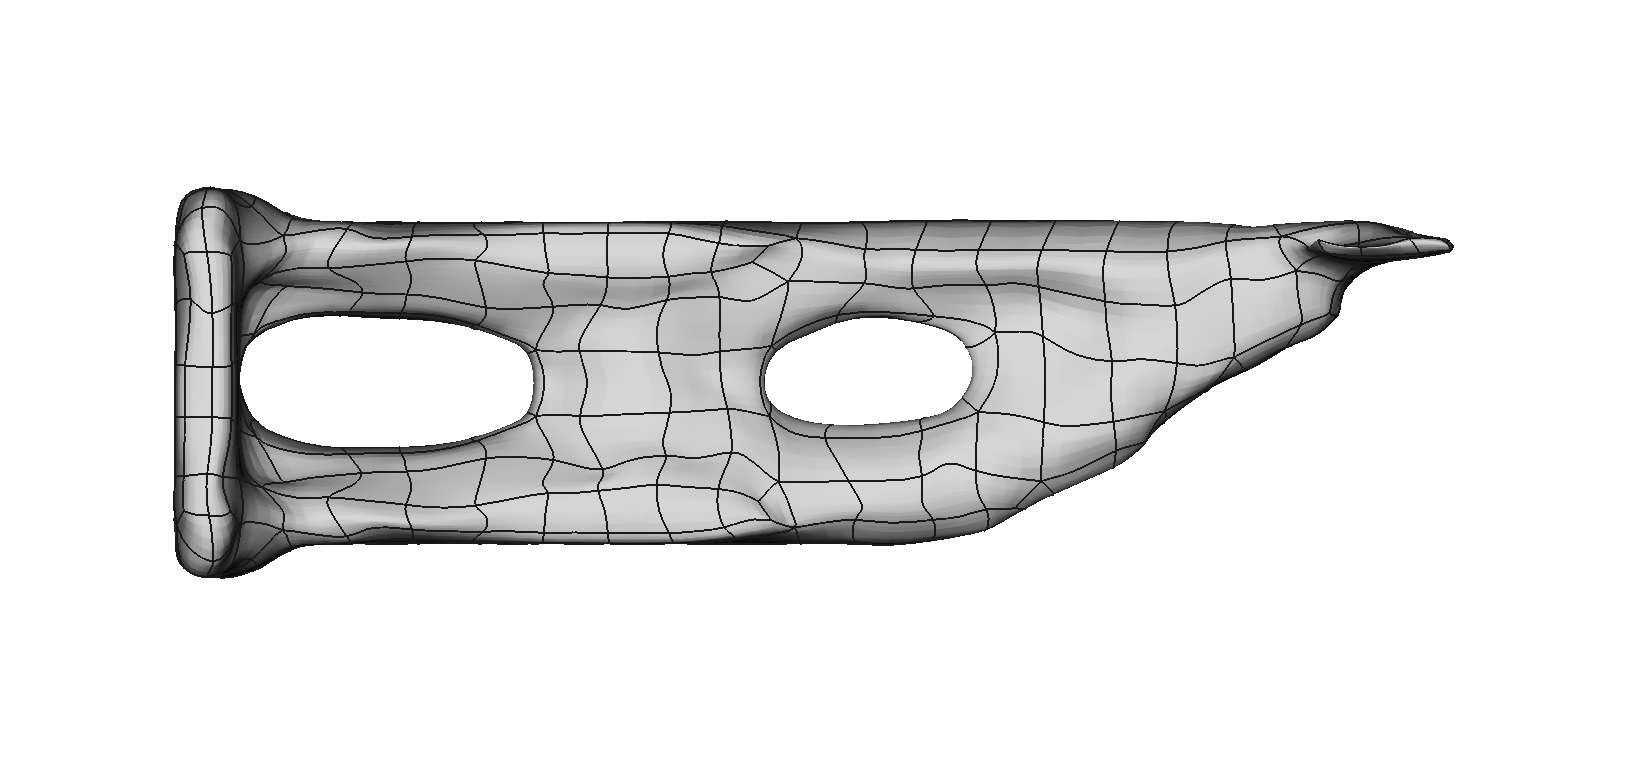
\includegraphics[scale=0.1]{Pictures/CADO_Overview/Back2CAD5.png}};
        \path[thick, ->] (N4) edge [bend left] (N6) node[yshift=0cm, xshift = 2.7cm]{(d)};
        \path[thick, ->] (N6) edge [bend left] (N5) node[yshift=-1cm, xshift = 0.1cm]{(e)} node[yshift=3cm, xshift = -8.7cm]{(f)};
        \end{tikzpicture}
        \caption{The workflow of CADO}
        \label{fig:pipeline}
	\end{center}
\end{figure}

\section{From \acs{CAD} to Voxels}
\todo[inline]{OpenCascade Class UML diagramm }
\todo[inline]{reading geometries, voxelise to VoxelBoolDS, Writer classes }
\label{sec: CADToVoxels}
One of the hurdles with most state-of-the-art open source topology optimization tools is their input format, where many of them (including ToPy, our topology optimizer of choice) require input to be specified as a 3-dimensional voxel grid. Presence (or absence) of material in these voxels is defined by a boolean variable, and boundary conditions are imposed on the appropriate locations. An example of voxelized data can be seen in \autoref{fig: voxelOpenCascade}. %Since there is a variety of toolboxes available which are able to perform a voxelization of common CAD input files, we did not implement one of our own but rather adapted one of the open source tools. %This section describes how we overcame this hurdle of converting CAD representations to voxelized input.
\begin{figure}
\centering
  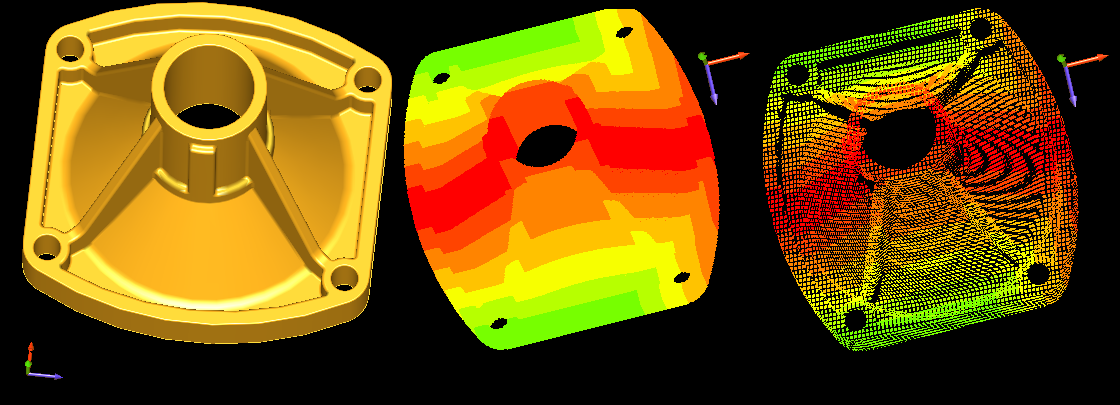
\includegraphics[scale=0.3]{Pictures/CADToVoxel/voxels_wp_image005.png}
\caption{A shape and its voxel representation. \emph{Leftmost picture}: The original parametrized shape. \emph{Rightmost picture}: The voxel representation. Picture from OpenCascade \cite{OpenCascade}.}
\label{fig: voxelOpenCascade}
\end{figure}

\label{sec:CVMLCPP}
In the variety of toolboxes available for voxelization, we decided on the \emph{Common Versatile Multi-purpose Library for C++} (CVMLCPP). This is a collection of mathematical algorithms whose objective is "to eliminate this redundancy by offering high-quality implementations of commonly needed functionality" \cite{CVMLCPP}. The library offers an easy-to-use voxelizer, which we use for conversion of CAD input to a boolean voxel grid.

Another very popular open-source choice is the 3D modeling toolbox is OpenCascade \cite{OpenCascade}, a versatile library with huge amounts of functionality. Although this also offers a voxelizer, we decided that its additional functionality did not justify its disadvantages in size and cumbersome installation requirements on for example a linux system.
\begin{figure}
\centering
\begin{subfigure}{
  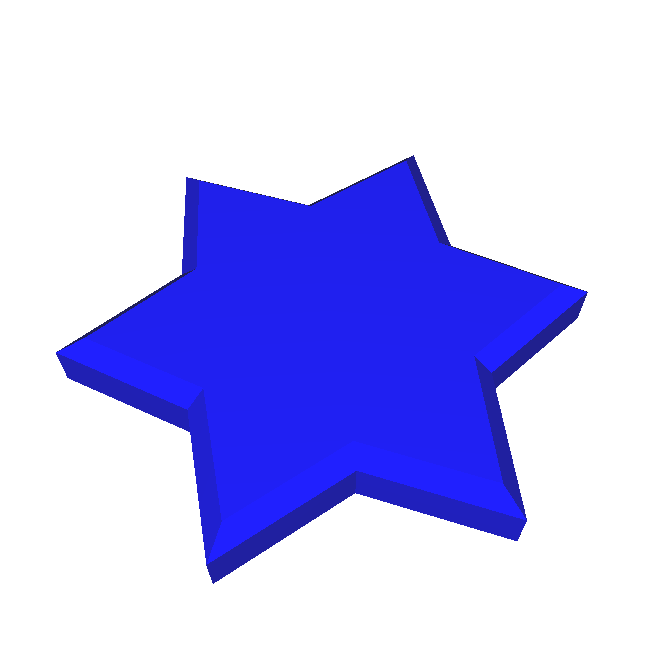
\includegraphics[width=.2\linewidth]{Pictures/STLToVoxels/Star_STL.png}}
\end{subfigure}
\begin{subfigure}{
  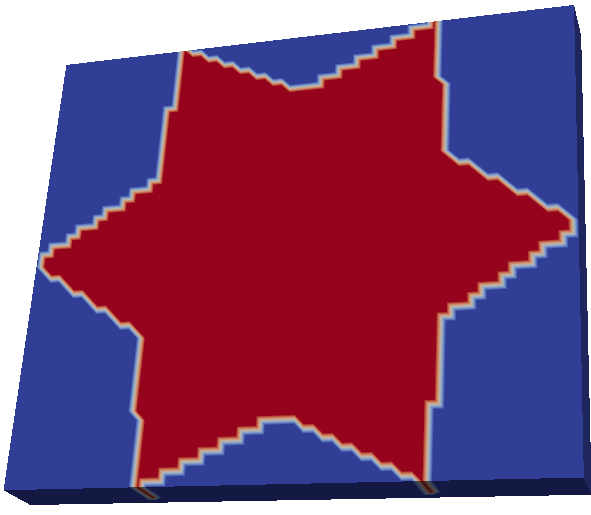
\includegraphics[width=.2\linewidth]{Pictures/STLToVoxels/Star_VTK_Trans.png}}
\end{subfigure}
\caption{The STL geometry of a star (left) and its voxelized form (right) obtained via the CVMLCPP voxelizer, visualized by Paraview \cite{Paraview}.}
\label{fig: voxelizerStar}
\end{figure}

In terms of implementation, the only thing required is the installation of the CVMLCPP library. The voxelizer is then included as a callable binary, that takes STL-file input (\autoref{subsub:STL}) and converts it to a .dat binary file with dimension and voxel information, with specifiable voxel size. An example result of using the voxelizer is shown in \autoref{fig: voxelizerStar}.
 %In the end, to voxelize a file given as .stl-input, we could just call 
%\begin{lstlisting}
%~/Path/To/CVMLCPP/bin/voxelize ./<stl_file>.stl <voxelSize>
%\end{lstlisting}
%where $\mathtt{<voxelSize>}$ is an integer declaring the size of a voxel. 


\section{Topology Optimization}
\label{sec:ToPy}
\todointern[inline]{Severin: Review}
Due to the good range of topology optimization software available, we decided to adapt an open-source topology optimizer to our needs, namely \emph{ToPy}.


ToPy \cite{ToPy} is a python library/program, written by William Hunter and documented in \cite{Hunter2009}, implementing the SIMP model and method described in \autoref{subsec:TopOpTheory}. It is based on the 99-line Matlab code by Sigmund's for minimum compliance \cite{sigmund200199}. The program can optimize the previously named problem types: minimum compliance, heat conduction and mechanism synthesis --- in 2D as well as 3D. It uses highly optimized open source python libraries such as Pysparse \cite{Pysparse} and Numpy \cite{Numpy}, leading to improved speed, porta- and scalability. %The whole program is steered by an input file which-- with the help of the documentation-- is straightforward to use and easy to adapt. %citation on pysparse and numpy


%In terms of our implementation, 
We use ToPy as a black-box topology optimizer. This means, we launch the program with an input file based on our scenario and let ToPy run. Next, as soon as the output is available, we proceed with the next step. The intention is to create separate modules to be able to plug in different solvers later on. In order to specify our input, we wrote an auxiliary program taking a voxelized CAD design provided by OpenCascade as input, outputting a .tpd file with geometry, load and fixture information in the format required by ToPy. 

Results of the topology optimization process can be seen in figure \ref{fig: topyStar}. Here, a star was given as input from a STL-file. We set the voxels in the star's points as fixtures, while we set a load in the middle, in the direction normal to the plane of the star. As can be seen, the optimization process "cuts" away unnecessary material in-between the corners and even in the middle of the material, returning an optimally stiff structure for the chosen remaining volume fraction. 
\begin{figure}
\centering
\begin{subfigure}[c]{.24\linewidth}
\centering
  
\includegraphics[width=\linewidth]{Pictures/TopOp/Star_Optimized0_Trans.png}
\end{subfigure}%
\begin{subfigure}[c]{.24\linewidth}
\centering
  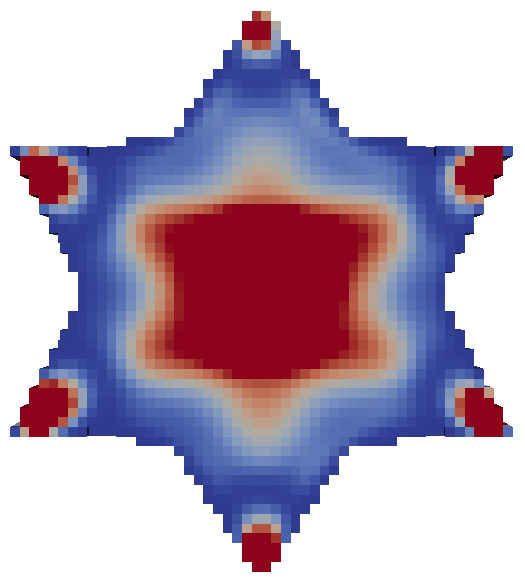
\includegraphics[width=\linewidth]{Pictures/TopOp/Star_Optimized2_Trans.png}
\end{subfigure}
\begin{subfigure}[c]{.24\linewidth}
\centering
  
\includegraphics[width=\linewidth]{Pictures/TopOp/Star_Optimized4_Trans.png}
\end{subfigure}
\begin{subfigure}[c]{.24\linewidth}
\centering
  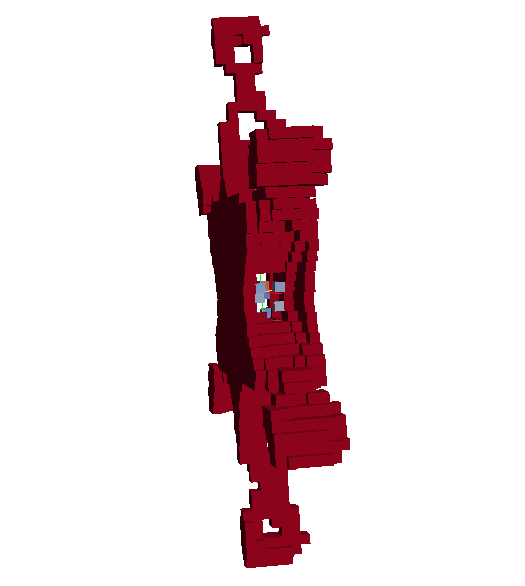
\includegraphics[width=\linewidth]{Pictures/TopOp/Star_Optimized5_Trans.png}
\end{subfigure}
\caption{Topology Optimization by ToPy \cite{ToPy}, with minimum compliance. \emph{From left to right}: increasing number of SIMP iterations until convergence. The star-shaped structure was given by an STL-file which was processed into input readable by ToPy, with fixtures in the corners, and a load in the middle. Throughout the SIMP iterations, one can see how material from the less dense regions (blue) is concentrated into denser regions (red) that carry the load. The last picture gives a rotated view, to illustrate how material has been eliminated even from the inside of the star. } %which volume fraction?
\label{fig: topyStar}
\end{figure}


As was mentioned above, surface extraction is an intermediate step after Topology Optimization and NURBS representation in order to facilitate the conversion. In terms of implementing the surface extraction, we used VTK.

%\subsection{VTK Toolbox}


%The VTK toolbox was used in order to implement the algorithms on our optimized data. It is a heavily object
%oriented toolbox. Our first approach was to use the built in Marching Cubes algorithm,
%nevertheless it did not work with our unstructured grid data. It just works for ImageData and
%PolyData . For structured and unstructured grids the tool to render the isosurface is the \textit{Contour Filter} tool. Unfortunately the documentation does not present which algorithm the tool uses. It
%can be inferred that it is an extended Marching cubes algorithm.

The VTK Toolbox is an open--source tool, providing algorithms for "3D computer graphics, image processing, and visualization" \cite{VTKToolbox}. Among the variety of tools, VTK offers algorithms that allow us to obtain a surface representation from voxel data. Among these algorithms, we could find Marching Cubes, Dual Contouring and also a Decimation method, which is useful for reducing the data size further for the NURBS-representation step.


%\subsection{Implementation}
Since \textit{Marching Cubes} algorithm only works with ImageData and PolyData, it is inapplicable to our case of unstructured grid data. For structured and unstructured grids the tool to render the isosurface is the \textit{Contour Filter} tool. Unfortunately, the documentation does not present which algorithm the tool uses. It can be inferred that it is an extended \textit{Marching Cubes} algorithm.
The \textit{Contour Filtering} works fine but the visualization of our data was still not possible
and an intermediate step was needed. We used the \textit{Implicit Modelling} tool which is a filter that
computes the distance from the input geometry to the points of an output structured point set.
This distance function can then be "contoured" to generate new, offset surfaces from the original
geometry. Although this approach allowed the visualisation, some crucial information was lost. In particular, holes are not represented in the final model.  
%It finally allowed visualization but it created one problem. Holes are lost in
%the process.

\begin{figure}
\centering
   \scalebox{0.4}{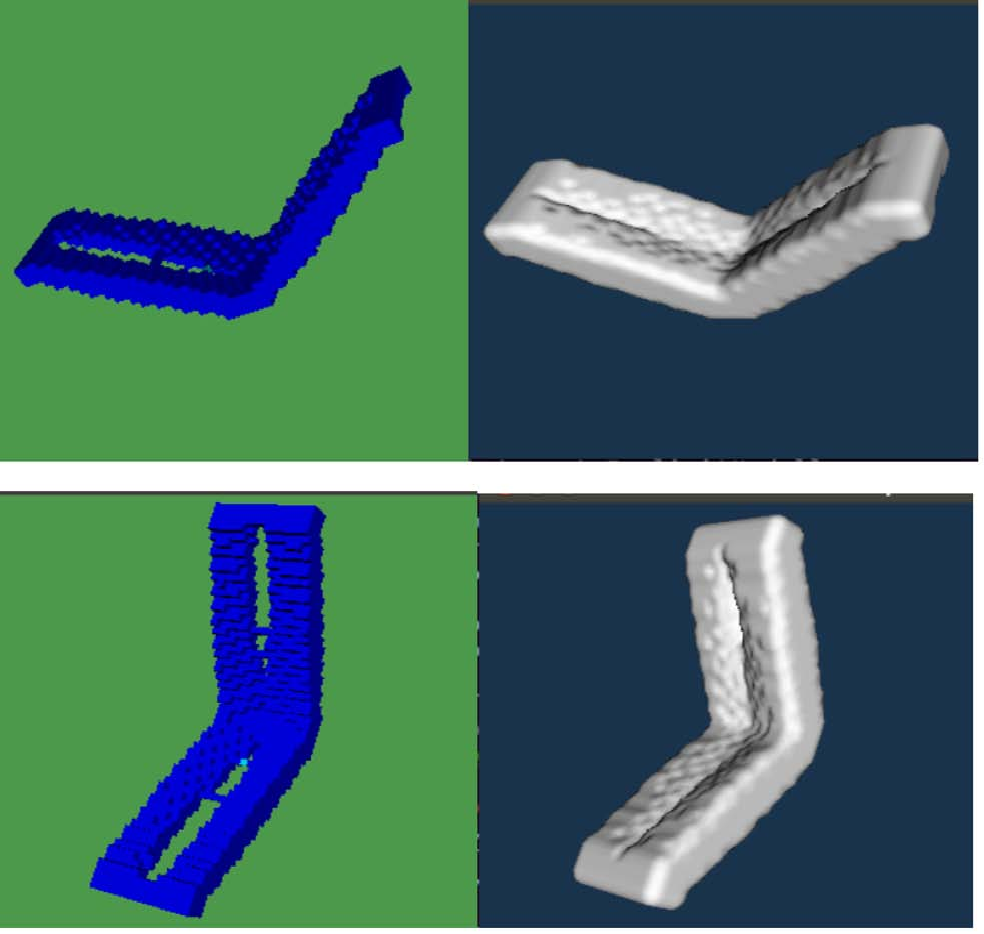
\includegraphics{Pictures/contouring.pdf}}\\
   \caption{Contour Filtering tool after Implicit Modelling}
   \label{fig:contouring}
\end{figure}

A further idea to solve this problem is to first convert the volume data into point data
and only then present it to the \textit{Contour Filtering} tool (\autoref{fig:contouring}).

In order to reduce computational costs of the following \textit{NURBS fitting} process, presented in the next section, we need to create a coarser mesh from the fine one. The number of triangles that represent the
isosurface can be reduced with the \textit{Decimation} tool. A smoothing step is necessary in between
to get the new connections right. The top part of figure \ref{fig:Decimation} shows a 50 \% reduction of the
triangles, a noticeable difference can not be perceived. On the lower part a 90 \% reduction is
obtained, it is nevertheless still difficult to see a difference. Triangle meshes can be easily
coarsened since there are many open source algorithms that simplify the triangles. VTK has the
decimation tool which works for 3D triangle data.

\begin{figure}
\centering
   \scalebox{0.4}{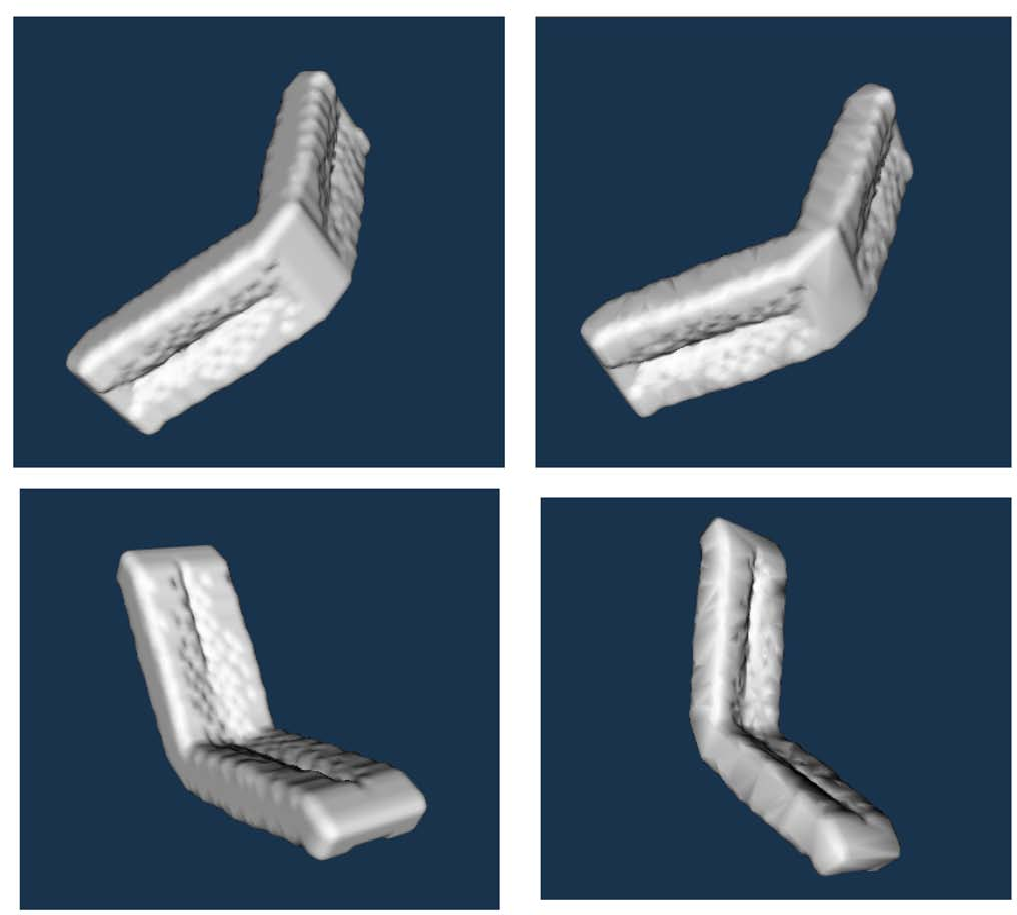
\includegraphics{Pictures/Decimation.pdf}}\\
   \caption{Decimation of triangles. \textit{Top:} 50\% \textit{Lower:} 90\%}
   \label{fig:Decimation}
\end{figure}


\section{From Parametrized Surface Points to NURBS Representation}
As of yet, there is no open-source software which provides the conversion from a \textit{mesh-based} geometry to NURBS representation. Hence, one of the main challenges of both the algorithmic and implementation part of this project has been to develop one from scratch. Due to a variety of possible approaches to tackle this problem (e.g. \cite{ eck1996automatic, becker2011advanced}), we therefore conducted extensive prototyping work in MATLAB \cite{MATLAB} to avoid cumbersome and time-consuming implementation overheads during the prototyping phase. Once the algorithms to be used had been finalized, the prototypes were implemented a non-proprietary language, Python.

Following the example of using Peters' scheme to fit NURBS smoothly to datapoints in \cite{eck1996automatic}, we did extensive prototyping to ensure the tractability of using Peters' scheme (see \autoref{subsec:peters}) for fitting a NURBS surface (see \autoref{subsub:petersleastsq}) in our settings. As mentioned above, these prototypes were done in MATLAB, and were also partly implemented in Python. 

Incorporated in these algorithms were also the least-squares fitting with a Fairness Functional term (see \autoref{subsec:fairnessthry} and \autoref{subsec:lsqfairness}) to ensure surfaces without unnecessary sharp wiggles.

In the following part of this section, the implemented algorithm will be shortly described, based on the theory and notations in \autoref{sec:NURBS} and \autoref{sec:LSQfitting}.

\subsection{Algorithm}
The algorithm is given information about a quadrilateral mesh of vertices ($\petersControlMeshVec \in \petersControlMesh$), how they are connected into quads ($\verticesof{\hat{f}}, \forall \hat{f} \in \petersFaces$) as an ordered list of four vertex indices, and how they are parameterized (parameters $(u_\lsDataPoint, v_\lsDataPoint)$ and on which quad $\hat{f}\in\petersFaces$).   roughly proceeds as follows:
\begin{itemize}
\item The information obtained from the Dual Contouring scheme is 
\item Implementations of the algorithm to calculate these \Bez point coefficients, as well as plotting them for debugging and visualisation
\item \Bez curve and surface evaluation via calculating the coefficients on each \Bez control point from a set of parameters
\item Algorithms to extract the necessary datapoints and parameters from the result data of the \acf{DC} algorithm in \autoref{ssec:DC}, using geometric conversions where necessary, and ignoring unusual datapoints
\item An algorithm for using the four above algorithms to assemble the total coefficient matrix in \autoref{eqn:petersminimisation} in \autoref{subsub:petersleastsq}
\item An application of MATLAB's built-in least squares minimisation tool to fit the resulting network of \Bez patches to the extracted surface.
\end{itemize}
A sample result, the fitting of a surface to a toroidal shape defined implicitly for the \acs{DC} algorithm is shown in \autoref{fig:fittingStructures}.


\begin{figure}
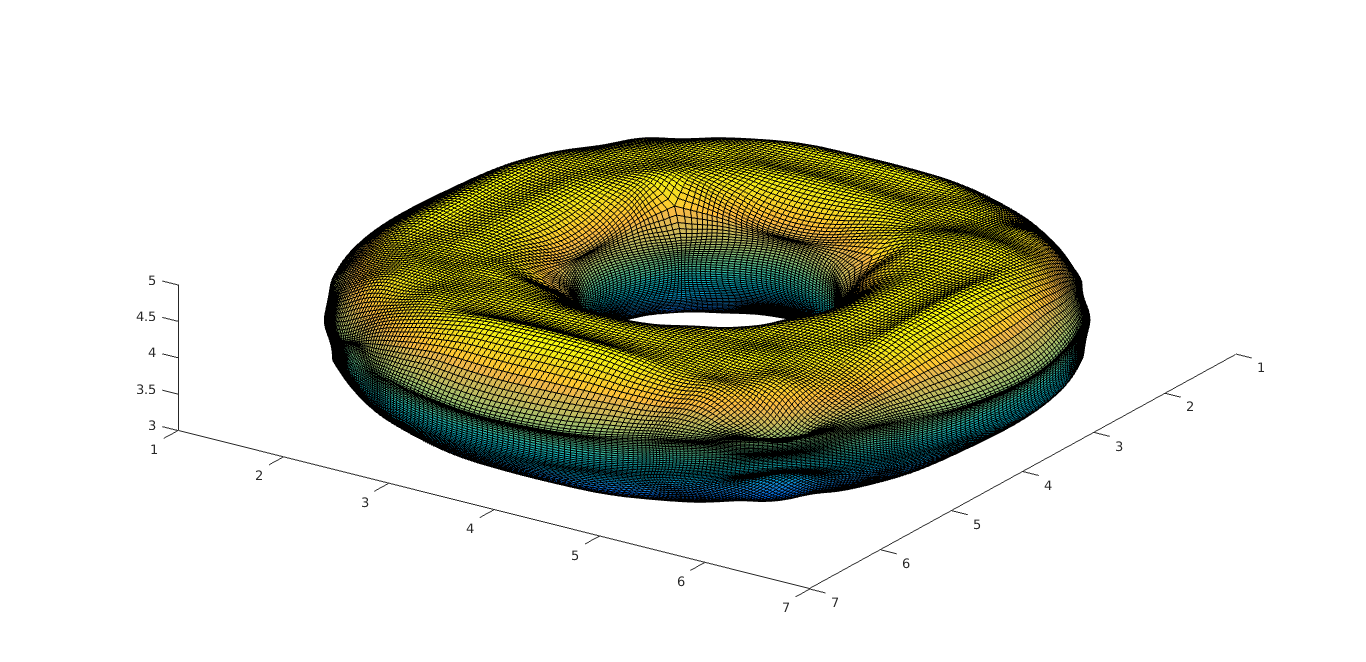
\includegraphics[width = \textwidth]{Pictures/NURBS/torus_from_DC.png}
\caption{A sample result from the Peters' scheme least-squares minimisation surface fitting, using the data provided by the \acs{DC} algorithm for an implicit function describing a torus. The grid lines on the figure are following the constant lines of each parameter value. As they follow the patch edges, corners where other than 4 coarse quads are meeting can be recognized, as for example on the middle of the far side of the torus, on the side that's facing the viewer.}
\label{fig:fittingStructures}
\end{figure}
\todourgent[inline,author=Benni]{From Bezier patches to NURBS using degree elevation. Add this to theory and implementation or only here?}




\section{From NURBS to Standardized CAD File Format}
\tododone[inline,author=Benni]{Should be rather short. Just explain that we use FreeCad Python interface. Severin finished this section, complain to me! =)}
In order to create standardized CAD files from previously computed B-Spline control points, the scripting functionality offered by FreeCAD is employed. Almost all functions of FreeCAD can be called using a python script, which allows to utilize FreeCAD functions within the automatized tool-chain. \cite{FreeCAD}

%installation path
Thus, the implemented python script is structured as follows: 
\begin{enumerate}
\item The installation path is specified and FreeCAD modules are imported separately
\item A new document is opened and B-Spline patches are consecutively created according to control points from Peters' scheme
\item  The object is reoriented to revert coordinate changes imposed by Topy (see section \ref{sec: ToPyInputConstruction})
\item Geometric constraints are enforced with boolean operations in FreeCAD  
\item The active object is exported as step file.
\end{enumerate} 






\section{Graphical User Interface}
\label{sec:gui}
In order to make user interaction with CADO as simple as possible, Graphical User Interface was implemented using the Qt5.4 \cite{Qt} framework. 
The interface allows to enter all necessary files and parameters without typing them into the command line. In particular, user chooses only the main \textit{.step} file and then, if all other files were named according to the naming convention (see \autoref{sec: CADToVoxels}), user just has to check the checkbox for specifying fixtures or the optimization domain (see \autoref{fig:mainWindowParameters}).

All necessary input parameters for the topology optimization can be entered through the input fields:
\begin{itemize}
\item Force Scaling - parameter for the force scaling (see \autoref{sec: CADToVoxels}).
\item Resolution - parameter for calculating the voxel size for the voxelization. Voxel size is then equal to $2^{-(Resolution - 1)}$. Hence, by increasing the resolution user reduces the length of the edge of a voxel by half.
\item Volume Fraction Limit - the fraction of the volume to be kept after the topology optimization process by ToPy (see sec. \ref{sec:ToPy}).

\end{itemize}
\todo{Do we subtract one from it now or not???}
All necessary input parameters for the surface fitting (see \autoref{sec:LSQfitting}) can be entered through the input fields:
\begin{itemize}
\item Smoothing - parameter for the fairness functional (see \autoref{sec:NURBS})
\item Coarsening - the number of coarsening steps in Dual Contouring(see \autoref{ssec:parametrization}).
\end{itemize}

After all parameters are specified, the pipeline can  be executed without any interaction with the user. After the process has finished, there is an option to lunch FreeCAD directly from the GUI  and view the results.

\begin{figure}[h]
\centering
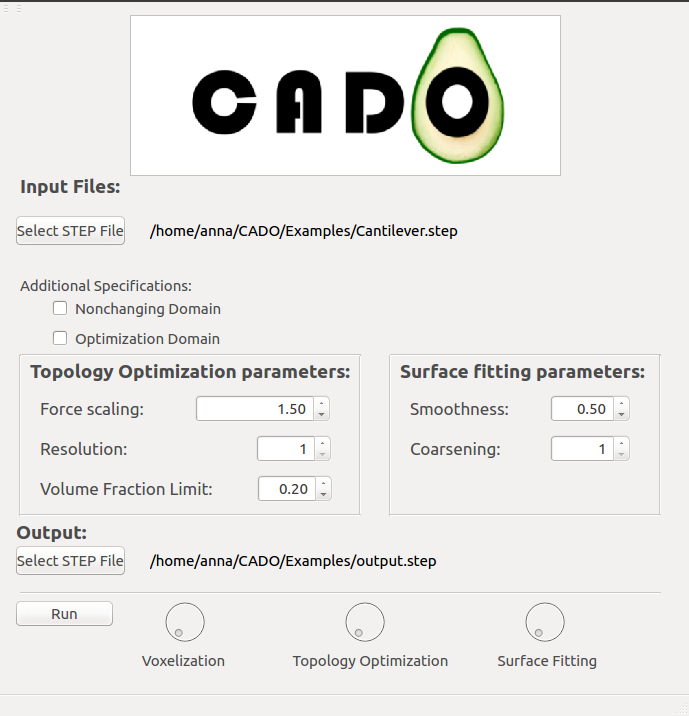
\includegraphics[scale=0.5]{Pictures/CADO_mainWindowParameters.png}
\caption{CADO User Interface showing file input and parameters for topology optimization and surface fitting. During execution of the program, the dials at the bottom indicate progress of the operation}
\label{fig:mainWindowParameters}
\end{figure}
\todointern{Saumi: Add more meat in the caption}


